\documentclass[class=ctexart,crop=false]{standalone}

\usepackage{amsmath,amssymb,enumitem,empheq,tkz-euclide,
diagbox,wrapfig,pgfplots,geometry}
%\geometry{a4paper,scale=0.9}
\pgfplotsset{compat=newest}
%\usepgfplotslibrary{external}
%\tikzexternalize
\renewcommand\parallel{\mathrel{/\mskip-2.5mu/}}

\newcommand\px{\mathrel{/\mkern-5mu/}}  %平行
\newcommand\pxeq{\mathrel{\vcenter{     %平行且等于
\ialign{\hfil##\hfil\crcr
$\scriptstyle\px\!$\crcr
\noalign{\nointerlineskip\vskip1pt}$=$\crcr}}}}

%\setCJKmainfont{SimSun}       %设置西文字体为times new roman
%\setCJKsansfont{SimSun}             %设置中文字体为宋体
%\setCJKmonofont{STKaiti}
%\setsansfont{TeX Gyre Termes}            %设置typewriter family中文字体为楷体
%\setmonofont{TeX Gyre Termes}

\usetikzlibrary{calc,intersections,through,backgrounds,patterns}
\newcounter{para}
\newcommand\mypara{\par\refstepcounter{para}\thepara.\space}%设置typewriter family西文字体为times new roman
\newcommand*\circled[1]{\tikz[baseline=(char.base)]{
            \node[shape=circle,draw,inner sep=1pt] (char) {#1};}}

\newcommand{\rnum}[1]{\romannumeral #1}
\newcommand{\RNum}[1]{\uppercase\expandafter{\romannumeral #1\relax}}
\begin{document}
    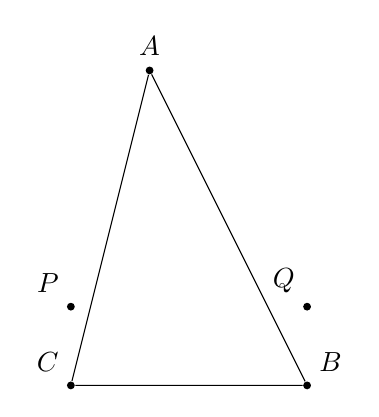
\begin{tikzpicture}
        \node[label={[label distance=0.005cm]90:{$A$}},circle,fill,inner sep=1pt] (A) at (0,4) {};
        \node[label={[label distance=0.005cm]60:{$B$}},circle,fill,inner sep=1pt] (B) at (2,0) {};
        \node[label={[label distance=0.005cm]120:{$C$}},circle,fill,inner sep=1pt] (C) at (-1,0) {};
        \node[label={[label distance=0.005cm]120:{$P$}},circle,fill,inner sep=1pt] (P) at (-1,1) {};
        \node[label={[label distance=0.005cm]120:{$Q$}},circle,fill,inner sep=1pt] (Q) at (2,1) {};
        \draw (A)--(B)--(C)--(A);
    \end{tikzpicture}
\end{document}